\documentclass[12pt]{article}
\usepackage[backend=biber,natbib=true,style=alphabetic,maxbibnames=10]{biblatex}
\usepackage[utf8]{vietnam}
\addbibresource{/home/nqbh/reference/bib.bib}
\usepackage{tocloft}
\renewcommand{\cftsecleader}{\cftdotfill{\cftdotsep}}
\usepackage[colorlinks=true,linkcolor=blue,urlcolor=red,citecolor=magenta]{hyperref}
\usepackage{amsmath,amssymb,amsthm,float,graphicx,mathtools}
\allowdisplaybreaks
\newtheorem{assumption}{Assumption}
\newtheorem{conjecture}{Conjecture}
\newtheorem{corollary}{Corollary}
\newtheorem{definition}{Definition}[section]
\newtheorem{dinhnghia}{Định nghĩa}[section]
\newtheorem{example}{Example}
\newtheorem{hypothesis}{Hypothesis}
\newtheorem{lemma}{Lemma}
\newtheorem{notation}{Notation}
\newtheorem{note}{Note}
\newtheorem{principle}{Principle}
\newtheorem{problem}{Problem}
\newtheorem{proposition}{Proposition}
\newtheorem{question}{Question}
\newtheorem{remark}{Remark}
\newtheorem{Rule}{Rule}
\newtheorem{theorem}{Theorem}
\usepackage[margin=2cm]{geometry}

\title{Some Thoughts On Learning, Teaching, {\it\&} Research\\Vài Suy Nghĩ Về Việc Học, Việc Dạy, {\it\&} Nghề Nghiên Cứu}
\author{Nguyễn Quản Bá Hồng\footnote{E-mail: {\tt nguyenquanbahong@gmail.com}. Bến Tre City, Việt Nam.}\and Nguyễn Quản Trung Nhân}
\date{\today}

\begin{document}
\maketitle
\begin{abstract}
	This note consists of some pieces of my writing, which are able to be shared and I am willing to share, in order to sharpen my flow of thoughts, to balance my scientific work via various aesthetic forms, \& to track psychologically and mentally my transitions from boyhood to manhood if there is any.
\end{abstract}
\setcounter{secnumdepth}{4}
\setcounter{tocdepth}{3}
\tableofcontents

%------------------------------------------------------------------------------%

\section{Preliminaries}

\subsection{Disclaimers}
We, the authors, in the role of the narrator of this novel, clearly state that
\begin{itemize}
	\item Any character names mentioned in this piece of writing is purely imaginary.
	\item If there is any coincidence, so that a person in real life in the three-dimensional physical space, denoted by $\mathbb{R}^3$, feels offended. I can apologize, if I feel necessary, but I take no responsibility.
\end{itemize}
Chúng tôi, các tác giả, trong vai trò người kể chuyện, tuyên bố rõ ràng rằng:
\begin{itemize}
	\item Bất kỳ tên nhân vật nào trong câu chuyện này đều là thuần hư cấu.
	\item Nếu xảy ra bất cứ sự trùng hợp nào, để mà 1 người nào đó ngoài đời thực trong không gian vật lý 3 chiều, tạm ký hiệu là $\mathbb{R}^3$, cảm thấy tự ái. Tôi có thể xin lỗi nếu cảm thấy cần thiết nhưng từ chối nhận trách nhiệm.
\end{itemize}
Lúc còn làm về động cơ đốt trong (combustion engines), có 1 giai đoạn tôi phải học luật \& các vấn đề đạo đức (ethical issues) phát sinh phòng trường hợp research output của đề tài mà tôi làm bị ứng dụng sai vào mục đích quân đội (military purposes) hoặc dân dụng, làm gây thiệt hại nghiêm trọng. Lúc đó tôi chỉ thấy phiền mà không hiểu cho lắm. Nhưng trải qua vài chuyện thì thấy nó cần thiết thật, với nhiều cái hay lắm (thảo nào mấy cuốn sách luật ở Đức dày 1 cách quái dị). Nên tôi nghĩ điều đó cũng cần phải nêu rõ ở đây, khi mà các vấn đề về tâm lý chưa bao giờ là dễ dàng để tiếp cận, để đề phòng các tình huống xấu nhất. Có lẽ thời gian tôi phải đọc tài liệu về luật \& làm các workshop về scientific ethics (i.e., nonfiction) triền miên, ngốn cả thời gian làm nghiên cứu raw của tôi, cuối cùng sau vài năm cũng được bù đắp theo cách dị hợm nhất có thể: tôi dùng nó cho fiction novel -- tiểu thuyết hư cấu. What a joke!

\subsection{Notation}

\begin{itemize}
	\item $\mathbb{R}^3$: three-dimensional physical space. Không gian vật lý 3 chiều.
	\item $\mathbb{C}^3$: three-dimensional imaginary space. Không gian ảo, tưởng tượng 3 chiều.
	\item $\Psi$: Psychology. Tâm lý học.
	\item $\Phi$: Philosophy. Triết học.
	\item Bhr: Behavior. Hành vi.
	\item Env: Environment. Môi trường mà 1 con người hiện đang sinh sống \& phát triển.
	\item $P$: a typical person. 1 con người điển hình. P cũng là viết tắt của Point, có thể hiểu như 1 điểm trong không gian Euclidean $\mathbb{R}^3$. Kiểu hiểu này có lợi khi xét tương tác giữa 2 hay nhiều người với nhau cũng tương tự như tương tác giữa các hạt trong lý thuyết kinetics\footnote{Tôi được học môn này của lớp Master 2 ở Rennes, Pháp.}, see, e.g., \cite{Tartar2008}.
\end{itemize}

\subsection{Outline}
3 phần chính của tiểu thuyết này là bàn về việc học, bàn về việc dạy, bàn về nghiên cứu, theo thứ tự trưởng thành dần theo chiều phát triển của 1 người. Nhưng tôi chợt nghĩ lại có khi thứ tự đó không chuẩn cho lắm, thứ tự mà tôi cho là đúng chính là bàn về nghiên cứu, bàn về việc dạy, \& cuối cùng là bàn về việc học. Nghe có vẻ ngược ngạo, nhưng từ những trải nghiệm của tác giả trên con đường nghiên cứu chuyên nghiệp, tôi nhận ra có nhiều thứ quá giá hơn ngoài văn phòng nghiên cứu. 

\section{Ignition}
Christmas Eve, Winter 2020. Berlin, Germany. In the imaginary world $\mathbb{C}^3$ instead of the real physical world $\mathbb{R}^3$.

Hắn thấy mình đang mệt nhoài, toàn thân rã rời, lê bước trở về phòng riêng trong 1 student studio ở Alexanderflatz\footnote{ \textit{Alexander Square}: a large public square \& transport hub in the central Mitte district of Berlin, reputedly the most visited area of Berlin, see \href{https://en.wikipedia.org/wiki/Alexanderplatz}{Wikipedia{\tt/}Alexanderplatz}.}, Berlin--Mitte, sau buổi tối thân mật cùng đồng nghiệp chung team nghiên cứu của hắn. Nói là đồng nghiệp nhưng thật ra không hắn làm viêc chung 1 đề tài. Nếu là 1 công việc bên mảng công nghệ hoặc kinh doanh chắc có lẽ sẽ khác. Đây là công việc nghiên cứu. Mỗi người trong team sẽ chịu trách nhiệm 1 mảng nghiên cứu riêng, dù chung 1 research theme, nhưng khó mà làm chung với nhau được. Đấy là cái thất bại đầu tiên của hắn: hắn không tương tác được với đồng nghiệp để tạo ra ý tưởng mới. Nhưng có nên trách hắn không? Hắn chỉ là 1 nghiên cứu sinh bậc tiến sĩ, đồng nghiệp của hắn toàn postdoc -- nghiên cứu sau tiến sĩ, khi mà họ đã rành mảng của họ \& sẵn sàng tương tác với các đồng nghiệp trong nhóm lẫn những đồng nghiệp khác nhóm, thậm chí các giáo sư head research group, thì đây là 1 mảng hoàn toàn mới với hắn. Hắn cần thời gian để cày kiến thức nên -- nhưng đúng ra thì thời gian không cho phép. Hắn đang trong giai đoạn cuối của 1 đề tài sắp nghiệm thu mà các người tiền nhiệm của hắn đã bỏ hẳn.

Ít ra thì hắn cũng có 1 bài toán nhỏ với thầy của hắn được xuất bản trên 1 tạp chí toán phổ thông nổi tiếng của Đức, tựa tựa tạp chí Toán học \& Tuổi trẻ ở quê nhà của hắn. Hắn mừng lắm. Chẳn phải xuất bản khoa học, nhưng cũng được tính KPI (key performance indicator) để giảm bớt áp lực công việc.

Sáng Giáng sinh năm ấy hắn dậy sớm, ra siêu thị mua đồ ăn ngon. 

There have been many broken pieces of memories in his head. Good memories. Bad memories.

Hắn nhớ lại cha hắn. Chợt hiểu ra vài thứ. Có lẽ hắn không có khả năng để tạo hạnh phúc cho người khác. Nếu có khả năng về mặt thuần tình cảm thì cũng chả có vị thế về vật chất. Hắn chấp nhận rồi buông bỏ.

A dark student room in , opposite the main Police station. No sound. No sign of life. He can't feel anything from himself. He is not presented.

Hắn chợt choàng tỉnh dậy sau cơn mê man, đầu óc mụ mị, nhức như búa bổ. Mình phải tính tay cho xong -- hắn nấu 1 ít rồi ngồi vào bàn \& làm việc. Hắn không muốn những cảm xúc. Hắn cho những thứ đó là cấm kỵ của 1 người làm khoa học. Quá ủy mị. Quá mềm yếu. Hắn cứ lờ đi mặc dù tiềm thức cảnh báo hắn.

\begin{quote}
	God. It's just a fucking simple work. Just get it done. Move to something else.
\end{quote}
Hắn ước gì phiên bản tương lai của hắn sẽ quay trở về giúp hắn, cho hắn 1 lời khuyên hay ho nào đấy hoặc đấm 1 cú trời giáng thẳng vào bộ não ngây thơ của hắn để hắn tỉnh ngộ, thậm chí thức tỉnh. Chả có ai giúp hắn cả. A contradiction in both his drinks and his subconscious mind. He works in mathematics so long to avoid contradiction, now it comes to his lifestyle, his psyche.

Hắn say xưa làm việc. Phòng bên hì hục làm tình. Sự thăng hoa hắn tự cho là đã tìm thấy trong công việc \& sự khoái cảm của bộ trai gái phòng bên hòa hợp, át đi tiếng siren còi hú inh ỏi của đồn cảnh sát. Nhịp nhàng. Giống như vũ điệu reo hò soran, 1 nét văn hóa đẹp của người Nhật.

He knock a drink of beer. He didn't like wines. Then he drank a lot of black coffee, the pure one.

Beer so he can forget bad shits, coffee so he can focus on the good. Actually a side effect of coffee helps him shit well too. The cure for all the sittings long hours labor work.

Thay vì chịu sự cô đơn, hắn thỏa hiệp với vài con người thuần lợi dụng. 

What is missing? What pieces of the picture of life do I miss? A little self-estem? A little understanding how life works?

Hắn tự huyền hoặc bản thân với 1 trí nhớ tốt, sự ảo tưởng sức mạnh về món quà mà hắn được ban tặng.

Nah, these things so difficult. I get back to my mathematics, my calculus.

What is the point of all of this?

Oh oh, so if I can do all these math, my father's liver cancer will disappear right? he can live right? He can be normal again like nothing happens right?

Fucking bullshit. All of this. Purely fucking bullshit.

Hắn tự hỏi liệu Chí Phèo đã cảm giác thế nào vào cái lúc hắn vừa đi vừa chửi. Cái làng Vũ Đại ngày ấy. Vãi đạn thật.


Then he felt awake. Something inside him awoke. He was not sure about it but totally aware of its presence.

This is a very different battle - the one I can't win now. If you lost a battle within yourself then how the hell you can win any other battle?

He had worked so hard to be able to take all the responsibility the only job offered to him, then he got claimed to be lazy \& irresponsible in many senses.



This is the battle he will lose no matter how.

Do I want to die as a good man? Like my father? No, I want to die as a wise man. 1st, I need to confront my stupidities.

The man who lost his faith in God finds a way to get insight. The journey of revealation begins.

\cite{Tolle2022}

Oppenheimer Homocunlus

You mean Newton is the fuck boy of science? Yo, no! The player. Like Mozart - the player of musical instruments. Here I mean the player of formulas \& concepts.

My conscious mind has still been working with this idea no matter how I deny \& destroy all pieces of my writings. The day my teacher die, the day I remember my father die. Consonant echoes from the past into the present. 

It is about the passion.

Power of concentration -- black fist in JJK.

\begin{center}\it
	Feeds the dying light, and brings me back to life\\
	Let the darkness lead us into the light 
\end{center}
Then the most dangerous intrusive thought won:

Hay là mình tạm ngưng làm toán mà thử làm nhà văn nhỉ? -- You're fucking kidding me right? Don't fool yourself. Joke on all of us.

Winter that year so cold, colder than before. He felt the damn cold in his own mind \& own heart.

He has no literary gift, not any gift for conceptual thoughts, just some average mathematical computation skills, not abstract enough to become a pure mathematician, not complex enough to become an applied mathematician. Who can he become then?

But the day his son, if he has any, ask him about these, what kind of father he is then?

I don't know what the fuck do you want. I really have no idea. \& I am so fucking tired to be pretentious. Listen. Pick your pieces up.

Solitude is inevitable.

So he starts to fight his primal fear, in the realm of literary -- word analysis, and psychology -- emotion analysis.

Maybe he never nail it, the kind of thoughts \& writings he always wants to pursue. But it is still a good try, a way to live aesthetically, spiritually, which means to be able to live properly.

\section{An Initial Configuration}

\subsection{Rules}
Mỗi người $P$ (abbr., person) có một xuất phát điểm $\{P(t)\}_{0\le t\le t_0}$ khác nhau, được hưởng hoặc bị ép nhồi các nền tảng giáo dục khác nhau, sự tương tác với những người khác nhau, cùng vô vàn những chuyện \& những biến cố họ gặp trong suốt 1 cuộc đời hoàn toàn khác nhau, thành ra nền tảng nhận thức \& xu hướng phát triển nhận thức, cùng sự hình thành các cấu trúc niềm tin \& các hệ giá trị cơ bản cùng thế giới quan của mỗi người hoàn toàn khác nhau.

Quy tắc đầu tiên ở đây là không phán xét, công kích (e.g., dí trên mạng xã hội) bất cứ ai. Cũng không áp đặt ai, thậm chí cả việc áp đặt ai đó không được áp đặt người khác. Tạo cho người khác 1 cảm giác thoải mái tối thiểu khi tiếp xúc.

Quy tắc thứ 2 là không quá tò mò vào cuộc sống cá nhân của người khác, e.g., stalk in social media -- rình mò trên các nền tảng mạng xã hội, xâm phạm tài khoản  riêng tư cá nhân bất hợp pháp. Keep healthy boundaries for both.

\begin{Rule}[Reset]
	Một phản tư xa hơn trong tương lai có lẽ là chẳng có hành trình phát triển tự thân nào mà đủ sức chống chọi 1 cách hiệu quả với các tương tác xã hội cả, đặc biệt là các tương tác xấu \& các mối quan hệ độc hại (toxic relationships) cả. Khi đó thì tất cả các ghi chú ở đây sẽ bị xóa. Mọi thứ trở về cấu hình sống nhiều mặt để che giấu bản thân phổ dụng.
\end{Rule} 

\subsection{Goals}
This writing activity is one of many ways, which is likely to become the main one, to balance between my scientific work \& personal life. I believe some arts will be the tool.

Việc viết lách, theo mình nghĩ, bằng cách này hay cách khác, một lúc nào đó \& theo 1 cách tự nhiên nào đó, cũng sẽ tìm tới những kẻ thích suy nghĩ, những kẻ hay nghĩ nhiều, \& những kẻ mệt mỏi vì cái tật đó, e.g., nhà nghiên cứu, nghiên cứu sinh, các học giả, nói chung là những người làm trong mảng học thuật hoặc phải tiếp xúc nhiều với chữ. Tật hay tài thì chưa biết nhưng ắt hẳn việc viết dùng để sắp xếp mọi thứ trong đầu cho ngăn nắp thì không thể tránh khỏi đối với những người làm việc đầu óc nhiều.

%------------------------------------------------------------------------------%

\section{Combustion: Order \&{\tt/}vs. Chaos}

\begin{figure}[H]
	\centering
	
\includegraphics[scale=.5]{true_detective_galaxy}
	\caption{Credit: True Detective.}
\end{figure}
Source: {\sc Jordan B. Peterson} \textit{12 Rules for Life: An Antidote to Chaos} \cite{Peterson2018} với bản dịch \textit{12 Quy Luật Cuộc Đời: Thần Dược Cho Cuộc Sống Hiện Đại} \cite{Peterson2022a}, {\sc Jordan B. Peterson} \textit{Beyond Order: 12 More Rules for Life} \cite{Peterson2021} với bản dịch \textit{Vượt Trên Trật Tự: 12 Quy Tắc Cho Cuộc Sống} \cite{Peterson2022b}.

\subsection{Art \& Life}
We need arts for life.
\begin{quote}
	``Perfectly balanced. As all things should be.''
\end{quote}

%------------------------------------------------------------------------------%

\section{Towards the $\Psi$-Flow: Optimal Experiences}
Các tài liệu: {\sc Mihaly Csikszentmihalyi}, \textit{Flow: The Psychology of Optimal Experience} \cite{Csikszentmihalyi2008} với bản dịch \textit{Dòng Chảy: Tâm Lý Học Hiện Đại Trải Nghiệm Tối Ưu}. Also \cite{Csikszentmihalyi2013}.

\begin{definition}[$\Psi$-flow]
	``\emph{Flow} in \href{https://en.wikipedia.org/wiki/Positive_psychology}{positive psychology}, also known colloquially as being \emph{in the zone} or \emph{locked in}, is the \href{https://en.wikipedia.org/wiki/Mental_state}{mental state} in which a person performing some activity is fully immersed in a feeling of energized focus, full involvement, \& enjoyment in the process of activity. In essence, flow is characterized by the complete absorption in what one does, \& a resulting transformation in one's sense of time. Flow is the melting together of action \& \href{https://en.wikipedia.org/wiki/Consciousness}{consciousness}; the state of finding a balance between a skill \& how challenging that task is. It requires a high level of concentration. Flow is used as a \href{https://en.wikipedia.org/wiki/Coping}{coping} skill for stress and anxiety when productively pursuing a form of leisure  that matches one's skill set.'' -- \href{https://en.wikipedia.org/wiki/Flow_(psychology)}{Wikipedia{\tt/}flow (psychology)}
\end{definition}

\begin{dinhnghia}[Dòng chảy trong tâm lý học]
	\emph{Dòng chảy} trong tâm lý học tích cực, còn được gọi thông tục là \emph{ở trong vùng} hoặc \emph{bị nhốt}, là trạng thái tinh thần trong đó 1 người thực hiện 1 số hoạt động hoàn toàn đắm chìm trong cảm giác tập trung tràn đầy năng lượng, tham gia trọn vẹn, \& thích thú trong quá trình hoạt động. Về bản chất, dòng chảy được đặc trưng bởi sự tập trung hoàn toàn vào những gì 1 người làm \& dẫn đến sự biến đổi trong nhận thức về thời gian của 1 người. Dòng chảy là sự hòa tan của sự hành động \& ý thức; trạng thái tìm kiếm sự cân bằng giữa 1 kỹ năng \& mức độ thách thức của nhiệm vụ đó. Dòng chảy đỏi hỏi mức độ tập trung cao. Dòng chảy được sử dụng như 1 kỹ năng đối phó với căng thẳng \& lo lắng khi theo đuổi 1 hình thức giải trí phù hợp với kỹ năng của 1 người 1 cách hiệu quả. 
\end{dinhnghia}

%------------------------------------------------------------------------------%

\section{On Research -- Bàn Về Nghiên Cứu}

\subsection{Dirty tricks -- Các thủ đoạn bẩn thỉu}
Các thủ đoạn dưới đây cũng áp dụng trong môi trường văn phòng, \& các môi trường làm việc trong phòng kín.

\subsubsection{Giả vờ xin tài liệu}
Hắn thấy mình đang cặm cụi tính, chợt đồng nghiệp người Anh gốc Ấn của hắn hỏi mượn tài liệu. Hắn chả nghĩ nhiều, cứ gửi qua bản tiếng Đức, kèm luôn cả bản dịch tiếng Anh mà hắn tự soạn, thêm cả ghi chú cá nhân vào đó. Hắn chợt nhớ tới chị Thương, senpai trước hắn 2 khóa, lúc hắn học Master 2. Hắn may mắn được học bổng của 1 viện nghiên cứu Pháp, Henri Lebesgue centre de math\'ematiques\footnote{\url{https://www.lebesgue.fr/en}.}. Chị ta cũng hay xin đề thi \& tài liệu của hắn. Hắn chả nghĩ nhiều nên cho mượn tuốt. Mỗi lần đưa là chỉ sẽ nói đề khó quá, có khi chỉ làm không nổi, cười mỉm, rồi sau lưng hỏi điểm từng đứa. Hắn lúc đó tự hỏi:
\begin{quote}
	{\sc Hồng}[22. Master 2 student]: Sao chỉ làm nổi nhỉ? Mình thấy chuyện hốt giải nhất Olympic sinh viên toàn quốc còn dễ chịu hơn mấy cái đề master 2 này. Toàn mánh khóe, calculus trick đủ kiểu. Phải cày liên tục suốt vài năm mới nhớ đủ trick để làm nổi. Trong khi chỉ còn chưa biết là hàm $L^2$ thì được không cho giá trị tại 1 vài điểm. Chắc chỉ chỉ đùa cho vui. Chắc thế.
\end{quote}
Tất cả tài liệu hắn đưa cho chị ta, chỉ đều phán: ``Chị thấy cũng dễ mà.'' Hắn khá rành kiểu này, nên chỉ cười mỉm rồi cho qua. Hắn chưa bao giờ muốn gây chuyện.
\begin{quote}
	{\sf Thương}[25]: Chị sẽ nói thầy của tụi mình để em khỏi làm luận văn luôn.
	
	{\sc Hồng}[23] nghĩ trong đầu: Đ.M. cái con khốn học dốt tới mức không biết mình dốt mà hám quyền. Tối ngày làm mấy cái chuyện nói xấu, đâm thọt sau lưng người khác mà tỏ ra tốt đẹp. Lủng background giải tích thua cả 1 đứa licence năm nhất Đại học mà tự cho mình cái quyền đì, quyền hành xác cái thằng tự kiếm học bổng Master làm từng khâu từ làm hồ sơ vấn \'Etudes en France tới phỏng vấn Campus France. Làm bẻ mặt dân Việt Nam trước cả lớp toàn mấy thằng Pháp hệ ENS. Má nó cái con khốn. Fucking stupid controlling bitch.
\end{quote}
Đoạn, hắn im lìm, mặt cúi gầm, không chịu ngẩng lên. Mà đúng ra hắn không thể ngẩng lên. Có cái gì đó đang chết \& mục rữa bên trong hắn.
\begin{quote}
	{\sc Hồng}[23]: \& anh có biết điều khiến tôi vừa sợ, vừa phát điên, \& ám ảnh hơn là gì không?
	
	{\sc Hồng}[27. Therapist]: Anh cứ việc nói. Tôi sẽ lắng nghe.
	
	{\sc Hồng}[23]: Đó là khi tôi nhìn xung quanh cái bữa tiệc ấy, đợi ai đó cản chị ta hay nhắc khéo để ngăn cái hành động ngu xuẩn của chị ta lại. Thì ai nấy cũng nhìn tôi như cái việc tôi đáng bị như thế là hiển nhiên nhất trên trần đời. A fucking crowd of bullies. Tôi có làm gì sai chứ? Tôi chỉ tốt với nhầm người, \& nhẫn nhịn với sai người.
\end{quote}

\subsubsection{Verbal bullying -- Bắt nạt lời nói}

\begin{quote}
	{\sf Dương}[26]: Mày lấy cái cứt gì mà qua được tới đây hả thằng kia?
	
	Ai thèm thuê cái chó như mày? Mẹ chả có cái chó gì cả mà xin được học bổng.
\end{quote}
Hắn chợt hiểu ra cái chuyện hắn giấu nhẹm mấy giải Olympic toán sinh viên toàn quốc là sai. Trước những đứa dốt tới mức không biết họ dốt, hắn hoàn toàn bất lực. Giữ hòa khí á? Chung tay góp sức xây dựng cộng đồng đoàn kết lành mạnh á? Fucking bullshit.

Dần dần, hắn căm ghét những buổi ăn chung tưởng chừng như đoàn kết nhưng toàn mấy thủ đoạn tìm điểm yếu, vạch lá tìm sâu, tỏ vẻ thông minh thượng đẳng, rồi bợ đít xu nịnh nhau như 1 lũ ô hợp. - Toàn 1 lũ bộ tịch, lúc nào cũng tỏ vẻ bộ tịch đầy giả tạo -- hắn phán hệt như nhân vật chính trong tiểu thuyết \textit{The Catcher In The Rye} \cite{Salinger_catcher_in_rye} của {\sc Jerome David Salinger} (bản dịch \textit{Bắt Trẻ Đồng Xanh} \cite{Salinger_btdx}).

Từ 1 đứa cố gắng sống tốt, trở nên có ích để giúp đỡ mọi người, bất cứ ai cần giúp hắn đều sẵn sàng giúp, giờ đây hắn dần hắc hóa thành 1 kẻ khó chịu. Điều mà sau này hắn nhìn lại thì thấy đó là 1 lẽ tất yếu. Hắn phải giết chết hoặc ít nhất là hạn chế cái phần agreeable tới mức quá lành của hắn, bằng cách đặt ra ngưỡng tối đa -- maximum threshold -- thì hắn mới phát triển 1 cách lành mạnh được.

\subsection{Standards -- Các tiêu chuẩn}
It is kind of funny, ironic, and sarcastic that the author of this writing is a dropout PhD student from one of the best research institutes of applied mathematics in Germany.

Anyhow, it is also a good idea to see from the outside. The perspective of an outsider may reveal some light \& insight to a dark room.

\textsf{\textbf{Slogan}}: \textit{A single bad publication will lead to endless public humiliations}.

\begin{quote}
	{\sf Thọ}[26]: Anh muốn làm nghiên cứu khoa học ``thực chất'' á.
\end{quote}
Ý ám chỉ các xuất bản mà hắn đã làm là bẩn, mà thực ra tự bản thân hắn thấy nó không đủ chuẩn như hắn mong muốn.

Hắn cũng chả hiểu anh ta cho lắm, chỉ biết nhiều anh chị lớn tuổi hơn than phiền việc bị anh này nhìn đểu. Nhìn đểu là sao cơ chứ? Thôi, không liên quan tới hắn, nên hắn cứ kệ. Mà cái éo gì bất cứ course nào hắn học, thì anh ta đều bảo là dễ cả. Dễ á? Hắn cày muốn bụp mắt mà chưa thấy có cửa cạnh tranh với mấy anh chị ENS Paris chung lớp để điểm hắn không bị đôn xuống quá đáng.


\subsection{Philosophical methodologies}
Khi phải đối đầu với những thứ thật sự khó nhằn, hoàn toàn nằm ngoài hiểu biết hiện tại của 1 cá nhân, thì 1 cách khá đơn giản là bám víu vào những thứ đã biết rõ, dù có thể lặp đi lặp lại 1 cách đơn điệu \& nhàm chán, nhưng lại có trật tự để cân bằng với hỗn loạn -- tượng trưng cho những điều chưa biết \cite{Peterson2018,Peterson2022a,Peterson2022b}.

\begin{example}
	Dạy học bậc phổ thông trở xuống thì ``nhàn'', theo nghĩa là không cần phải nạp quá nhiều kiến thức mới, nhưng phải chú trọng về phương pháp dạy \& truyền đạt kiến thức 1 cách hiệu quả tới các học sinh. Nếu học sinh giỏi, tiếp thu nhanh thì khỏe. Gặp học sinh dốt hoặc đầu gấu thì mệt, đâm ra chán chường, cảm thấy phí phạm thời gian \& nguồn sức lực hạn chế của bản thân.
	
	Nghiên cứu thì lại khác. Trách nhiệm của nghiên cứu là phải đọc thật nhiều, nạp thật nhiều kiến thức để trau dồi bản thân mỗi ngày.***
\end{example}
[...]

Tạm phân loại học giả, theo ý cá nhân (sẽ bổ sung thêm):
\begin{itemize}
	\item Học giả làm các mảng, lĩnh vực năng động, với năng suất xuất bản ấn phẩm khoa học cao, thường được trích dẫn nhiều nhờ sự năng động của cộng đồng khoa học tương ứng.
	\item Học giả làm các mảng khó nhằn, trừu tượng, nên tần suất xuất bản ấn phẩm khoa học khá thấp, nhưng các bài này đều ở dạng nặng đô (hardcore), thường ít được trích dẫn vì kén độc giả. Nếu bài báo đó trở thành cornerstone thì lại được trích dẫn nhiều đến rất nhiều, na ná dạng benchmark cases for industrial purposes của loại 1 (data mẫu chuẩn để các người làm nghiên cứu R\&D ở các lĩnh vực công nghiệp dùng).
\end{itemize}
Ưu điểm của loại 1 là đi hội nghị thường xuyên. Mà đa số mấy hội nghị này giàu do dính đến công nghiệp hoặc dịch vụ số hóa (AI{\tt/}DL{\tt/}ML) nên chắc đồ ăn nhiều \& ngon, ít nhất cũng ăn đứt mấy bữa tiệc giản đơn gồm trà, cafe máy cùng vài cái bánh quy như các hội nghị toán lý thuyết ở Pháp mà hồi mình học Master (hay chỉ có mấy chỗ nằm ở rìa của Pháp là vậy nhỉ?). Mà thực ra lúc mấy giáo sư Toán thảo luận với nhau, thay vì nhắm nháp cafe \& ăn bánh quy, vài người lại say xưa thảo luận mà ăn (nhầm?) phấn trắng.

Chắc mình thuộc loại 2, hoặc ít nhất là mình tự ép bản thân thuộc loại 2 (nên gọi là \textit{giả học -- fake scholar} thì hợp hơn). Trong khi loại 1 thì tạo cảm giác năng động, tràn trề của sức trẻ, thì loại 2 hoàn toàn ngược lại, mà phần lớn là phải cày background khá nhiều \& nặng, \& 1 trong những cái mệt nhất nhưng rewarding nhất của loại 2 là làm các công trình khoa học liên ngành, kết nối các kết quả mạnh nhất của các lĩnh vực lý thuyết với nhau.

Có 1 bài viết phân loại học giả hay của GS. Nguyễn Tiến Zũng của ĐH Toulouse. Tiếc là sau khi GS Zũng hỗn chiến với bác  Phùng Xuân Nhạ thì website cá nhân \url{http://zung.zetamu.net/} của GS trước bị lỗi font \& giờ có lẽ đã bay màu.

\subsection{Trends \& Choices -- Các Xu Hướng \& Lựa Chọn}	

\begin{quote}
	{\sc Nhân}[23]: Thế anh có biết những sở thích thời học sinh của 1 người ảnh hưởng thế nào đến xu hướng các lựa chọn chuyên ngành trong tương lai của họ không?
	
	{\sc Hồng}[28]: Tôi không rõ lắm. Cụ thể sao?
	
	{\sc Nhân}[23]: Tui sẽ lấy ví dụ về ngành Toán. Vì nó là cái duy nhất tui rành, ít hơn là rành hơn ối thứ còn lại.
	
	Những học sinh thích giải phương trình, hệ phương trình ở Toán Sơ Cấp nhưng không thích Tin học thường sẽ có xu hướng chọn các ngành lý thuyết trừu tượng, như Đại Số, Hình Học Đại Số. 
	
	Những người thích bất đẳng thức ở Toán Sơ Cấp thường sẽ có xu hướng chọn hướng Giải tích, đặc biệt là hướng Phương Trình Vi Phân Đạo Hàm Riêng (Partial Differential Equations, abbr., PDEs) vì hướng này chủ yếu đánh giá (estimation), chặn (bound), i.e., các bất đẳng thức giữa các không gian hàm. Như vậy, xu hướng thích đánh giá các đại lượng liên quan tới các hàm sơ cấp ở Toán Sơ Cấp thường sẽ phát triển thành niềm đam mê việc đánh giá các đại lượng liên quan đến hàm hoặc các đối tượng toán học trừu tượng hơn.

	1 câu hỏi điển hình của các nhà Giải tích học (mathematical analysts) khi thảo luận các vấn đề toán học liên quan đến PDEs là:
	
	- \textit{Do you think it is smooth (or regular) enough? -- Anh nghĩ nó có đủ trơn (hay nhớt) không?}
	
	- \textit{It seems a little rough at the initial phase. But it will be smoother later. Oh, now it's already smooth enough for us. Let's do{\tt/}play with it. -- Nhìn có vẻ hơi thô trong giai đoạn đầu (màn dạo đầu?). Nhưng rồi nó sẽ trơn hơn thôi. Ồ nhìn này, nó đủ trơn rồi kìa. Nào, chúng ta cùng xử{\tt/}quất{\tt/}chơi nó (vấn đề giải tích này) thôi}.
	
	Hàm đối tượng trơn chưa đủ, để đặt tốt 1 bài toán, miền xác định, i.e., nơi hàm đó sống, phải đủ trơn nữa, tức là cái mép (boundary $\Gamma\coloneqq\partial\Omega$) của cái miền $\Omega$ phải đủ trơn để xài các công thức tích phân từng phần (integration by parts formulas or Green's identities) để tạo ra dạng yếu (weak formulation or variational formulation). Những miền quá thô, e.g., có các góc nhọn (rough boundaries with corners), kỳ dị (singularities), chỗ nhọn dễ bị đâm (cusps), có nhiều lỗ (holes) hoặc gai (thorns) sẽ không thích hợp để làm chỗ chơi đối với các nghiệm trơn, dẫu mấy cái nghiệm đó có trơn chùi cỡ nào đi chăng nữa, vẫn không đảm bảo an toàn để chơi với chúng. Safety 1st.
	
	Ngoài lề, dù hay thắc mắc với việc đòi hỏi các nghiệm trơn, nghiệm nhớt của phương trình vi phân đạo hàm riêng có đủ trơn, đủ nhớt hay không để mà có thể vô tư chơi với chúng, tuổi thơ của các nhà giải tích cho thấy họ không có liên quan đến bất kỳ về tình dục sớm kiểu con nít quỷ hoặc sống thử, hay lạm dụng tình dục nào cả. Cho nên việc đề xuất những khẳng định kiểu như của {\sc Sigmund Freud}, e.g., các nhà toán học loay hoay với câu hỏi đủ trơn thường có tuổi thơ liên quan đến các vấn đề tình dục sớm do cha mẹ hoặc người tình của họ không quan hệ kín đáo để cho con cái vô tình bắt gặp hoặc các sang chấn tâm lý do chịu lạm dụng tình dục từ sớm; hoặc lý luận kiểu {\sc Malcolm Gladwell} trong quyển \textit{Outliers: The Story of Success} \cite{Gladwell2008} hay bản dịch \textit{Những Kẻ Xuất Chúng: Cái Nhìn Mới Lạ Về Nguồn Gốc Của Thành Công} \cite{Gladwell_outlier} ngụ ý việc tiếp xúc 1 cách vô thức với các từ gợi hình (gợi dục) tác động đến tiềm thức sâu bên dưới ý thức dẫn đến xu hướng chỉ thích làm với các đối tượng đủ trơn hoặc cuồng với các khái niệm đủ nhớt, etc. là hoàn toàn không có sơ sở.
	
	{\sc Hồng}[28]: What is so wrong with you?
\end{quote}

\subsection{Signs -- Các Dấu Hiệu}

\subsubsection{Personal systems of notations, abbreviations, \& conventions}
Bộ (tuple), tập hợp (set), hay hệ thống các ký hiệu, cách viết tắt, \& các quy ước cá nhân -- a personal set{\tt/}system of notations, abbreviations, \& conventions -- của 1 nhà khoa học tự nhiên thiên về lý thuyết hơn là về tính toán engineering thuần ứng dụng, e.g., nhà toán học (mathematicians), nhà vật lý (physicists), nhà khoa học máy tính (computer scientist), etc. là dấu hiệu đầu tiên cho biết trình độ của họ. Đơn giản vì các môn khoa học này có 1 đặc thù là đòi hỏi độ nhất quán (consistency) cực kỳ cao cho nên 1 hệ thống ký hiệu nhất quán, không mâu thuẫn, tiện dụng, không tạo ra bất kỳ sự mơ hồ, mờ mập (confusion) sẽ phản ánh phần nào trình độ của họ. Đấy là dấu hiệu dễ nhận biết đầu tiên -- nhưng còn xa so với mức phán xét -- của 1 người làm khoa học giỏi hoặc ít nhất là có 1 người thầy, người hướng dẫn giỏi.

Riêng các nhà hóa học (chemists) thì có lẽ họ được quy định chung bởi các danh pháp quốc tế như International Union of Pure and Applied Chemistry (abbr., IUPAC)\footnote{\url{https://en.wikipedia.org/wiki/International_Union_of_Pure_and_Applied_Chemistry}.} nên không{\tt/}chưa thể dùng hệ thống ký hiệu cá nhân để đánh giá sơ bộ. Có lẽ mình nên kết thêm vài đứa bạn chuyên ngành Hóa để hiểu thêm (vừa đủ).

Thus, a good advice for young science students: Build, polish, and perfect endlessly your personal system of notations and conventions so well that it will fit perfectly to any of, or at least most of, your research fields. Then you can effortlessly attack each of them, connect them, play with the interaction between them and beyond, and even foresee the hidden structure in the realm of abstractness.

Lời khuyên (tự thân) này na ná câu trích dẫn sau của Abraham Lincoln về việc đầu tư khâu chuẩn bị kỹ lưỡng:
\begin{quote}\it
	``Give me 6 hours to chop down a tree and I will spend the 1st 4 sharpening the axe.'' -- {\sc Abraham Lincoln} (1809--1865) -- 16th President of the United States (1861--1865)
\end{quote}

\subsubsection{Consistency -- Sự nhất quán}

\begin{question}
	Liệu có nên (dấn thân) theo 1 nghề cố định, không chịu{\tt/}thèm nhảy nghề không? 
\end{question}

\begin{figure}[H]
	\centering
	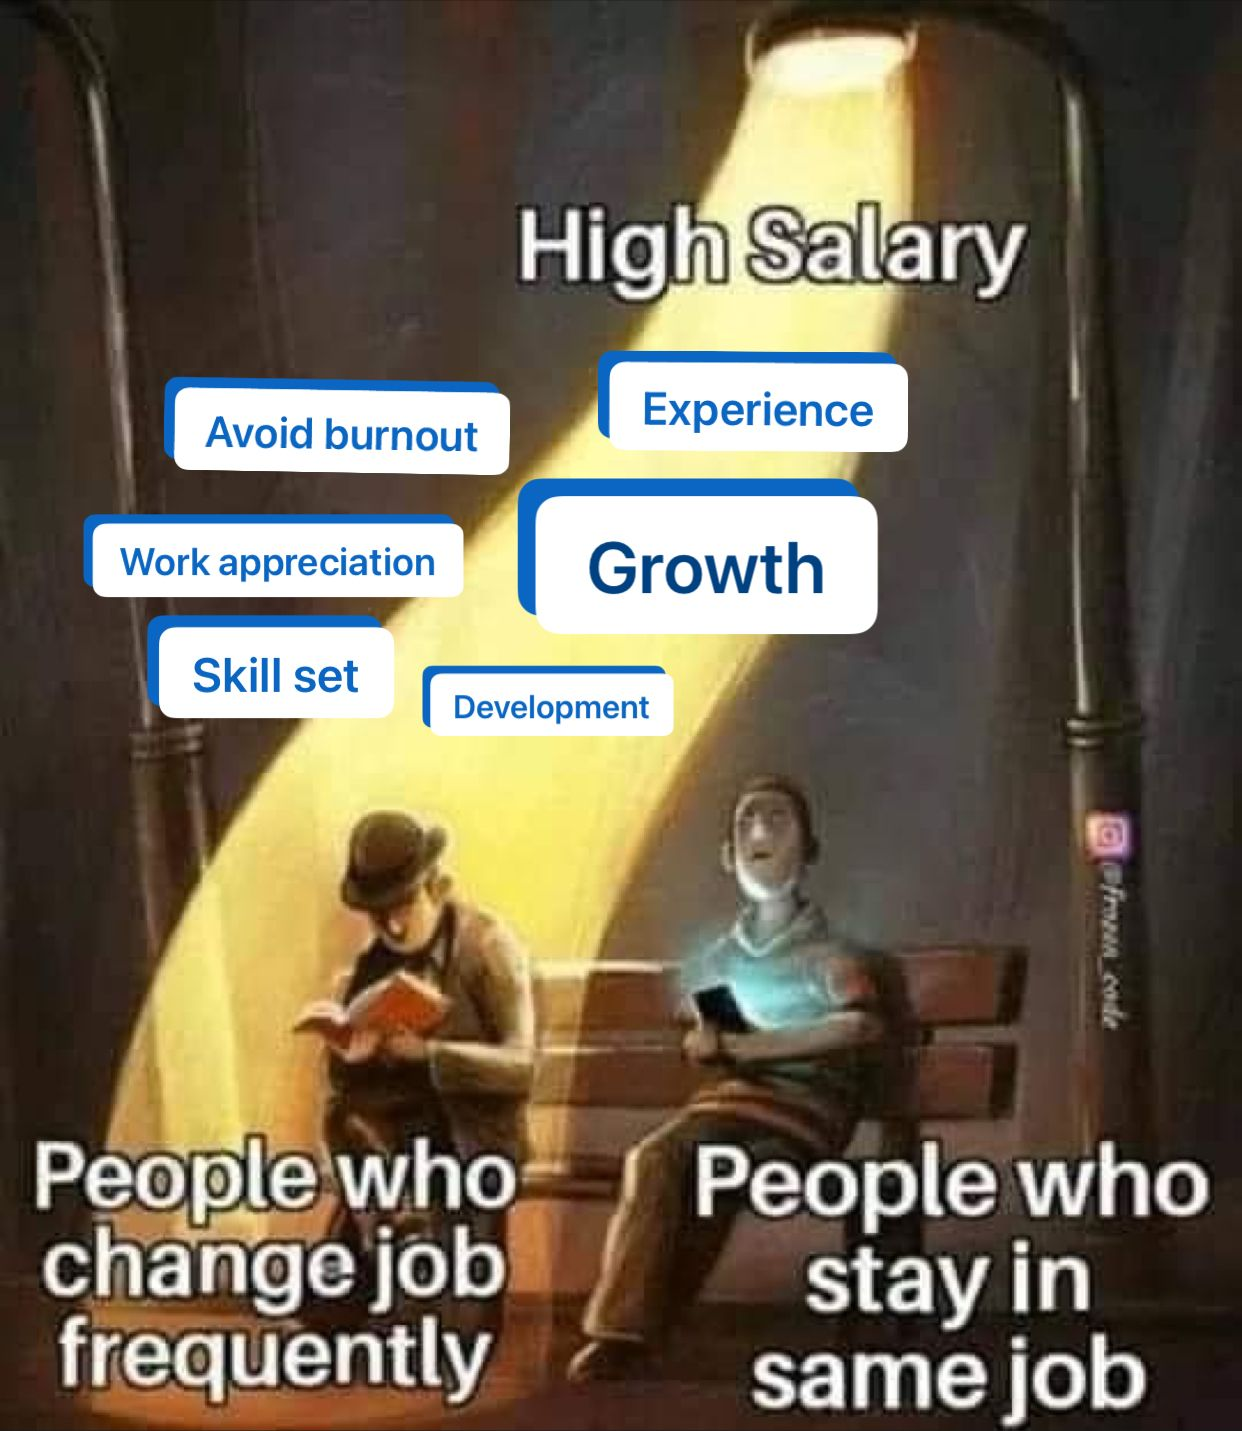
\includegraphics[scale=.15]{high_salary}
	\caption{Credit: \href{https://www.linkedin.com/posts/judy-soloai_i-didnt-learn-this-in-school-i-learned-activity-7089014937494179840-jTze/}{Linkedin{\tt/}Judy Soloai{\tt/}I didn't learn this in school}.}
\end{figure}
Hiển nhiên 1 câu hỏi khó muôn thở. Khó chịu lẫn khó nhằn theo nhiều nghĩa. Nghĩa thứ nhất là nó không rõ ràng, \& sự không rõ ràng đến từ việc bản thân nó phụ thuộc vào quá nhiều yếu tố không thể xác định hết như các yếu tố về phương diện vật chất, e.g., lương, tài chính; cũng như các yếu tố về phương diện tinh thần, e.g., ý nghĩa công việc, cân bằng công việc--cuộc sống (work-life balance), sự phát triển cá nhân, cùng sự tương tác lẫn nhau giữa các yếu tố trong 2 phương diện đó; \& nếu lùi xa hơn nữa về quá khứ thì chúng cũng phụ thuộc vào nhiều yếu tố ban đầu của 1 cá nhân như điểm xuất phát mà bố mẹ mang lại, hoàn cảnh như khả năng tài chính của gia đình, sự ủng hộ từ dòng họ, \& ảnh hưởng của các mâu thuẫn, xung đột, lục đục nội bộ trong 2 môi trường nền tảng đó.

Tôi không hề nghĩ sẽ cố trả lời 1 cách hoàn hảo câu hỏi này hay giải quyết vấn đề này. Đồng ý là tôi ngu, nhưng chưa ngu đến mức vậy. Chưa kể có bất kỳ câu trả lời nào không (no guarantee of existence), nếu có thì cũng không hề có câu trả lời duy nhất (even if the existence is assumed, the nonuniqueness is still valid), cũng như chưa \& sẽ không chả có câu trả lời nào sẽ thỏa mãn hết tất cả các phương diện giá trị được suy xét ở \textit{biểu diễn phân hoạch các giá trị \& ý nghĩa của cuộc đời} (\textit{a decomposition of values \& meanings in life}) sẽ được xét đến trong Sect. \ref{sect: bullshit theory on live}: \textit{A Bullshit Theory on Living -- 1 Lý Thuyết Nhảm Nhí Về Việc Sống}.


\subsubsection{Accuracy{\tt/}Precision -- Tính chính xác}

\subsubsection{Simplicity -- Sự giản đơn}
We use simplicity to fight difficulty. We do not add more unnecessary complexities and redundancies to the war because if we do so, we will have to fight ourselves, our entanglements.

\subsubsection{Minimality -- Sự tối giản}
\cite{Chi2022}.

\subsubsection{Vigor -- Khí lực, sức mãnh liệt}

\subsubsection{Rigour -- Tính chặt chẽ}

\subsubsection{Visionary -- Nhìn xa trông rộng}

%------------------------------------------------------------------------------%

\section{On Learning -- Bàn Về Việc Học}
It is never about how many books you read. It is about how you comprehend some \& how deep you can connect them.

\cite{Long2021}.

Decomposition:
\begin{itemize}
	\item Những điều ta chưa biết.
\end{itemize}

%------------------------------------------------------------------------------%

\section{On Teaching -- Bàn Về Việc Dạy}
Tôi gặp Hồng [nam, 27 tuổi] đang loay hoay viết về buổi trò chuyện của hắn với các thầy cô giáo cũ dưới quê.

\begin{quote}
	{\sc Hồng}[28]: Anh định viết thế nào?
	
	{\sc Hồng}[27]: Khó. Chả dễ. Viết lung tung cho đủ ý thì dễ, mà cho hay, cho trơn tru, đọc bắt tai thì khó quá xá.
	
	{\sc Hồng}[28]: Nếu dạng trò chuyện, tâm sự thì anh có thể tham khảo phong cách đối thoại trong 2 cuốn sách \textit{Dám Bị Ghét} \cite{Ichiro_Fumitake2022a} \& \textit{Dám Hạnh Phúc} \cite{Ichiro_Fumitake2022b} của 2 tác giả Nhật Bản \textsc{Kishimi Ichiro \& Koga Fumiake}.
	
	{\sc Hồng}[27]: Nội dung gì nhỉ?
	
	{\sc Hồng}[28]: Bàn về thuyết tâm lý học trường phái Adlerian. Nguyên bản là cuốn \textit{The Science of Living} \cite{Adler2013} của \textsc{Alfred Alder}.
	
	{\sc Hồng}[27]: Để tui đọc thử. Hy vọng không phải mấy cái học thuyết nhảm địt chỉ lý thuyết suông mà không tí thực tế.
\end{quote}

Nghe lời tôi khuyên, hắn bắt đầu viết. Cụ thể như sau.

\subsection{Dạy Trẻ Vùng Quê}
Tui tình cờ trò chuyện với Nhân [nam, 26 tuổi], 1 gia sư dạy các môn Tự nhiên như Toán Lý Hóa Tin, bên cạnh công việc nghiên cứu chưa đâu vào đâu của hắn, ở 1 vùng quê hẻo lánh.
\begin{quote}
	{\sc Hồng}[27]: Thế anh thích dạy? Thích công việc gõ đầu trẻ?
	
	{\sc Nhân}[26]: Cũng không hẳn. Không thích cũng không ghét. Thích vài cái \& cũng ghét 1 đống cái. Ban đầu nghe lời chị nên thử dạy, do công việc nghiên cứu bế tắc, hết đường tiến nên tạm lui về. Bế tắc sao thì sau tui sẽ kể chi tiết. Giờ tập trung vô việc dạy cái đã. Không kể liền có khi mất hồi nào không hay.
	
	Trước tui có về trường cấp 3 cũ để tham gia dạy đội tuyển học sinh giỏi của tỉnh nhà, hồi năm nhất, năm 2 Đại học. Đội tuyển chỉ có 6 đứa, chứ chưa được 8 hay 10 như của mấy tỉnh mạnh như Sài Gòn hay Hà Nội. Mà được cái 6 đứa giỏi, ngoan, chịu làm bài. Tui thích lắm, với hồi trước mấy thầy có phụ tiền cho tui lúc tui bị bệnh nên coi như là báo đáp cái ơn.
	
	Dưới quê thì khác hẳn. Mẹ nó cái vùng không có khỉ để ho mà cò cũng chả thèm gáy. Đa số học sinh không được giỏi cho lắm, toàn mấy dạng báo báo, mà chả dạng báo nào giống dạng báo nào. Những đứa vừa giỏi vừa ngoan, đủ trình để tui dạy hết sức, chắc hiếm như đếm số ngón tay của 1 đứa bị cùi.
	
	{\sc Hồng}[27]: Anh cứ bình tĩnh, việc gì phải xỉ vả thế?
	
	
	
	Tùy vào dạy ai, dạy cái gì, \& dạy ở mức độ nào.
	
\end{quote}

\begin{quote}
	- Sao mấy thầy cô cứ khó chịu chuyện yêu đương? Người lớn chả hiểu gì cả.
	
	{\sc Hồng}[27]: Đấy là góc nhìn của bạn. Còn trẻ tui cũng thế. [...]
	
	Rồi cô ấy tự sát với đứa con trong bụng. Thế bạn còn muốn sống thử không?
\end{quote}

Yondu Rabit


%------------------------------------------------------------------------------%

\section{A Bullshit Theory on Living -- 1 Lý Thuyết Nhảm Nhí Về Sống}
\label{sect: bullshit theory on live}
What is living? Why do we live? What to live for? Who to live with? How to live?

Maps of Meanings.

Let's hunt some low self-esteem.

Let's cook.

A little bit of trust. A little bit of betrayals.

A little bit of love. A little bit of denials.

Only take responsibility for whom deserved your responsibility.

\section{Miscellaneous}

\section{Acknowledgment}
We, the authors, apologize to save this part for the last. Set the acknowledgment switch is $\delta_{\rm ack}$. Đặt biến cảm ơn là $\delta_{\rm ack}$.

\begin{verbatim}
If project = fail
    take_responsibility = all
else, then {
    distribute_credit;
    thanks;
}
\end{verbatim}
Xin chân thành những người đã từng giúp, đã từng thương hắn đến tận ngày hôm nay. Cuộc hành trình mưu cầu hạnh phúc \& khám phá tri thức sẽ thật khó khăn nếu không có họ củng cố niềm tin của 2 tác giả. Xin cảm ơn chị Thảo, anh{\tt/}thầy Khang, thầy{\tt/}anh Khanh, thầy{\tt/}anh Chánh đã truyền động lực trên hành trình học Toán của 2 tác giả. Xin cảm ơn cô Hạnh, cô Thư đã viếng đám tang của cha tác giả, để họ không bị nỗi sợ bị bỏ rơi nuốt chửng. Xin cảm ơn thầy Huynh, thầy Hải, thầy Liêm, thầy Quí, thầy Trọng, đã là những mẫu hình người thầy tuyệt vời để 2 tác giả bắt chước theo.

Bạn đọc có thể dễ dàng nhận thấy đây là 1 chủ đề vô cùng nhạy cảm, cực kỳ nguy hiểm. Nên nếu dự án này thất bại, thì đều do sự non nớt của 2 tác giả, không liên quan gì đến bất cứ ai giúp 2 tác giả.

%------------------------------------------------------------------------------%

\appendix

%------------------------------------------------------------------------------%

\printbibliography[heading=bibintoc]
	
\end{document}